% ----------------------------------------
% Chapter: Stand der Technik
% ----------------------------------------
\chapter{Stand der Technik}
\label{chap:stand_der_technik}

Der Begriff Tribologie ist nach \cite{bartz_2000} die Wissenschaft und Technik von aufeinander einwirkenden Oberflächen in Relativbewegung.
Sie beschäftigt sich mit Reibung, Verschleiß und Schmierung sowie Grenzflächenwechselwirkungen zwischen Festkörpern, Flüssigkeiten und Gasen (Abbildung \ref{fig:das_tribologische_system}).

% ----------------------------------------
% Fig: Das tribologische System
% ----------------------------------------
\begin{figure}[htb]
    \centering
    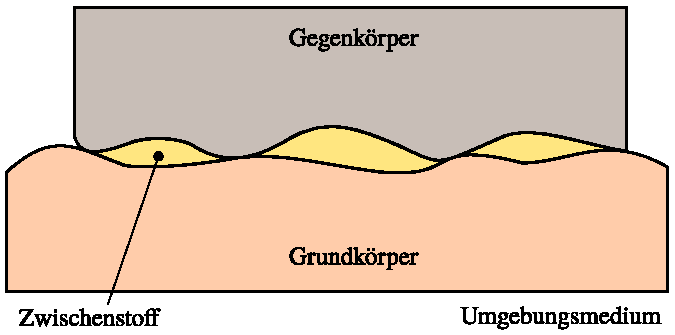
\includegraphics[]{./images/tribologisches_system.pdf}
    \caption{Das tribologische System\cite{wisniewski}}
    \label{fig:das_tribologische_system}
\end{figure}

Die vorliegende Arbeit beschäftigt sich vornehmlich mit dem ölgeschmierten Kugel-Scheibe-Kontakt.
Aus diesem Grund soll im folgenden kurz auf die Themen Schmieröle, Reibung und auf die elastohydrodynamischen Grundlagen eingegangen werden.

% ----------------------------------------
% Sec: Eigenschaften des Schmiermittels
% ----------------------------------------
\section{Eigenschaften des Schmiermittels}
\label{sec:eigenschaften_des_schmiermittels}

% ----------------------------------------
% Subsec: Viskosität
% ----------------------------------------
\subsection*{Viskosität}
\label{sub:viskositaet}
Viskosität, die auch als innere Reibung bezeichnet wird, ist die wichtigste Kenngröße eines Schmierstoffes.
Sie beschreibt die Zähigkeit von Flüssigkeiten und Gasen.
Je größer die Viskosität ist, desto dickflüssiger ist das Fluid und je niedriger die Viskosität, desto dünnflüssiger ist es.
Ein Modell des Parallelplattenversuchs veranschaulicht das Fließverhalten des Schmierstoffes, Abbildung \ref{fig:geschwindigkeitsprofil_parallelplattenversuch}.
% ----------------------------------------
% Fig: Geschwindigkeitsprofil in einem Parallelplattenversuch
% ----------------------------------------
\begin{figure}[htb]
    \centering
    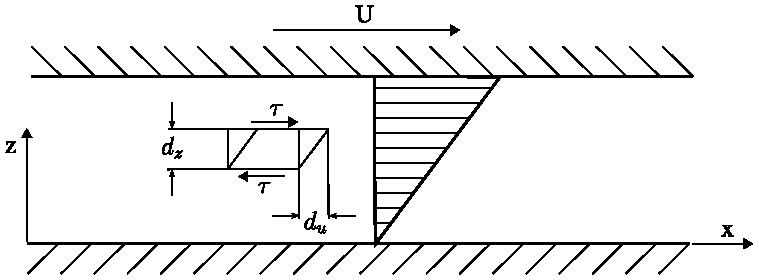
\includegraphics[]{./images/parallelplattenversuch.pdf}
    \caption{Geschwindigkeitsprofil in einem Parallelplattenversuch\cite{wisniewski}}
    \label{fig:geschwindigkeitsprofil_parallelplattenversuch}
\end{figure}

Für eine Newtonsche Flüssigkeit ist das Schergefälle $G = du/dz$ direkt proportional zur der Schubspannung $\tau$
% ----------------------------------------
% Eq: Schergefälle
% ----------------------------------------
\begin{equation}
    G = k  \tau
    \label{eq:schergefaelle}
\end{equation}

Die dynamische Viskosität (oder Viskosität) ist das Verhältnis von Schubspannung und Geschwindigkeitsgradient und ist der Kehrwert der Fluidität $k$ im Newtonschen Schubspannungsgesetz (\ref{eq:schergefaelle}).
% ----------------------------------------
% Eq: Dynamische Viskosität
% ----------------------------------------
\begin{equation}
    \eta = \frac{1}{k} = \frac{\tau}{G} = \frac{\tau}{du/dz}
    \label{eq:dynamische_viskositaet}
\end{equation}

Die kinematische Viskosität ergibt sich aus der dynamischen Viskosität durch die Division mit der Dichte des Fluids.
% ----------------------------------------
% Eq: Dynamische Viskosität
% ----------------------------------------
\begin{equation}
    \nu = \frac{\eta}{\rho}
    \label{eq:kinematische_viskotitaet}
\end{equation}

Im Si-Einheitensystem hat die dynamische Viskosität als Einheit $N  s/m^2$ oder $Pa  s$ und die kinematische Viskosität als Einheit $m^2/s$.
Ein Stoff hat die Viskosität $1~N  s/m^2$, wenn er in zwischen zwei Platten, die Größe von $1~m^2$ und einen Abstand von $1~m$ haben, befindet und man braucht $1~N$, um die zwei Platten gegeneinander mit einer Geschwindigkeit von $1~m/s$ zu verschieben.

\subsection*{Temperatureffekt}
\label{sub:temperatureffekt}
Die Temperatur hat eine große Effekt auf der Viskosität aller fließfähigen Stoffe.
Mit steigender Temperatur sinkt die Viskosität der Flüssigkeiten ab.
Diese Effekt kann experimentell mittel eines Viskosimeters und rechnerisch nach Cameron bestimmt werden.

Die einfachste Gleichung nach Reynold lautet:
% ----------------------------------------
% Eq: Dynamische Viskosität nach Reynold
% ----------------------------------------
\begin{equation}
    \eta = \eta_{s}  \ exp \left( -\beta  \Delta\phi \right)
    \label{eq:dynamische_viskositaet_reynold}
\end{equation}
%
wobei $\eta_{s}$ ist die Viskosität des Schmierstoffes bei der Temperatur $\phi_{s}$, $\eta$ ist die Viskosität des Schmierstoffes bei der Temperatur $\phi$, $\Delta{\phi}$ ist die Temperaturdifferenz ($\eta = \eta_{s} + \Delta{\phi}$) und $\beta$ ist die thermoviskose Konstante.\improvement{check the formel}
% ----------------------------------------
% Eq: Dynamische Viskosität nach Cameron
% ----------------------------------------
\begin{equation}
    \eta(\phi) = k_1  \ exp \left( k_2 / (\phi + 95) \right)
    \label{eq:dynamische_viskositaet_cameron}
\end{equation}

% ----------------------------------------
% Subsec: Viskositätsindex
% ----------------------------------------
\subsection*{Viskositätsindex}
\label{sub:Viskositaetsindex}
Die Temperaturabhängigkeit der kinematischen Viskosität eines Schmieröls wird auch von einem Viskositätsindex (VI oder KVI) beschreibt.
Der Viskositätsindex basiert auf einer Skalar, in der zwei unterschiedlichen Öltypen mit deutlich abweichenden Viskosität-Temperaturverhalten zugeordnet wurden.
Das Öl, das starke Veränderung der Viskosität ist, wird mit 0 oder LVI (low viscosity index) indiziert.
Das andere Öl wird mit 100 oder HVI (high viscosity index) gekennzeichnet.
Aus dem Vergleich der kinematischen Viskosität eines zu beschreibenden Öls mit diesen beiden Referenzölen bei $100^\circ$  ergibt sich dessen Viskositätsindex, Formel \ref{eq:viskositaetsindex}.
% ----------------------------------------
% Eq: Viskositätsindex
% ----------------------------------------
\begin{equation}
    VI~(oder KVI) = \frac{\nu_0 - \nu}{\nu_0 - \nu_{100}}
    \label{eq:viskositaetsindex}
\end{equation}
%
In der VI-Definition ist es angenommen, dass die Veränderung der Viskosität mit Temperatur von drei Ölen linear ist.
Die Linearisierung ist nach Walther (S\'{a}nchez-Rubio, et al.)\cite{sanchez-rubio} und wird in der Abbildung~\ref{fig:variation_der_viskositaet_mit_temperatur} für das Mineralöle dargestellt.
% ----------------------------------------
% Eq: kinematische Viskosität nach Walther
% ----------------------------------------
\begin{equation}
    \label{eq:kinematische_viskotitaet_walther}
    \log \log(\nu + 0,7) = A + B \log T
\end{equation}
%
% ----------------------------------------
% Fig: Naeherungsgleichung der Viskosität-Temperatur nach Walther
% ----------------------------------------
\begin{figure}[htb]
    \centering
    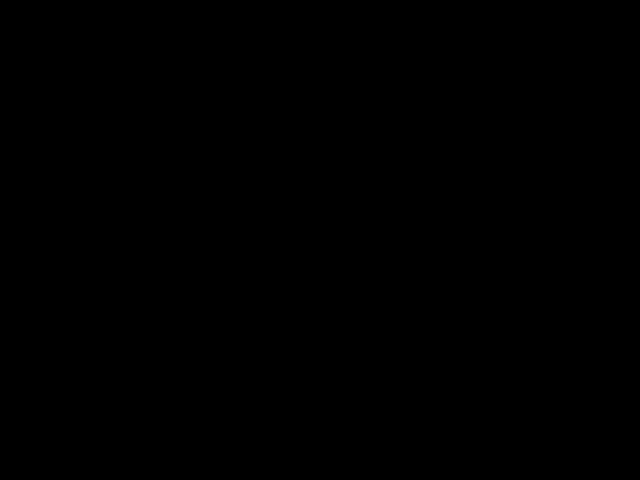
\includegraphics[width=5cm]{./images/blank_img.jpg}
    \caption{Variation der Viskosität mit Temperatur}
    \label{fig:variation_der_viskositaet_mit_temperatur}
\end{figure}
\improvement[inline]{Walther Linearisierung}

% ----------------------------------------
% Subsec: Einfluss von Druck auf Viskosität
% ----------------------------------------
\subsection*{Einfluss von Druck auf Viskosität}
\label{sub:einfluss_von_druck_auf_viskositaet}
Mit steigendem Druck nimmt die Viskosität aller Schmieröle zu.
% ----------------------------------------
% Fig: Viskosität - Druck - Verhalte
% ----------------------------------------
\begin{figure}[htb]
    \centering
    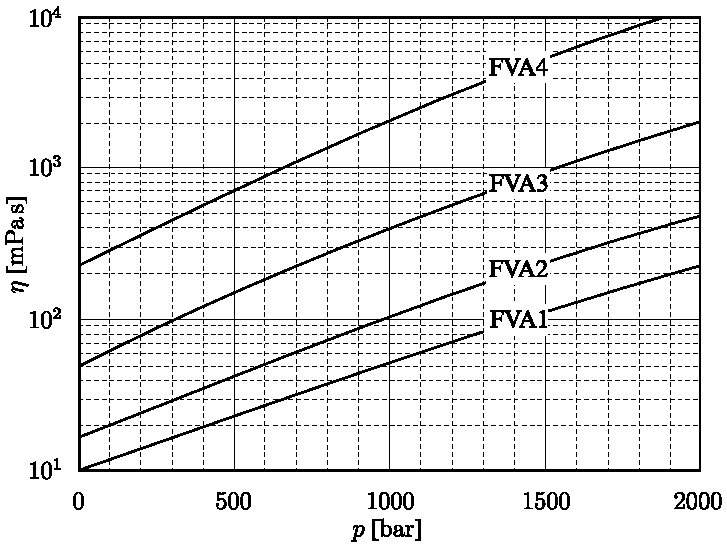
\includegraphics[]{./images/viskositaet_druck.pdf}
    \caption{Dynamische Viskosität in Abhängigkeit vom Druck}
    \label{fig:dynamische_viskositaet_in_abhaengigkeit_vom_druck}
\end{figure}
\improvement[inline]{Figure quelle ???}
%
Allerdings verändert sich das Schmiermittel unter dem für die EHD-Kontakte enormen Druck schlagartig.
Die Viskosität nimmt rapide zu und der Schmierstoff erreicht einem festen Zustand.
Nach Barus kann die Viskosität mit der unteren Formel berechnet werden
% ----------------------------------------
% Eq: Viskositätsindex
% ----------------------------------------
\begin{equation}
    \eta = \eta_0 \ exp(\alpha_p  p)
    \label{eq:dynamische_viskositaet_druck_barus}
\end{equation}
%
wobei $\eta_0$ die Viskosität beim Atmosphärendruck und $\alpha_p$ der Druckkoeffizient der Viskosität ist.
Für Mineralöle sind diese Parameter ungefähr

\begin{tabular}{llll}
    $0,001 \rightarrow 0,1$ & für & $\eta_0$ & $[Pas]$ \\
    $0 \rightarrow 4,0 \times 10^{-8}$ & für & $\alpha_p$ & $Pa^{-1}$
\end{tabular}

Leider liefert die Barus Gleichung einen zu großen Wert beim hohen Druck.
Eine genauer Gleichung wurde von Roelands\cite{roelands} vorgeschlagen
% ----------------------------------------
% Eq: Roelands Gleichung
% ----------------------------------------
\begin{equation}
    \eta(p, T) = \eta_0 \ exp \left[ (\ln{\eta_0} + 9,67)
                              \left( \left( 1 + \frac{p}{p_r} \right) ^z 
                              \left( \frac{T_0 - 138}{T - 138} \right)^{s_0} -1 \right) \right]
    \label{eq:dynamische_viskositaet_druck_roelands}
\end{equation}
%

Der Druckkoeffizient der Viskosität $\alpha_p$ ist nicht eine Konstante, sondern eine Funktion der Temperatur.
Diese Abhängigkeit wird in Abbildung~\ref{fig:druckkoeffizient_temperatur} für die Referenzöle der FVA gezeigt.
% ----------------------------------------
% Fig: Druckkoeffizient der FVA-Referenzöle in Abhängigkeit von der Temperatur
% ----------------------------------------
\begin{figure}[htb]
    \centering
    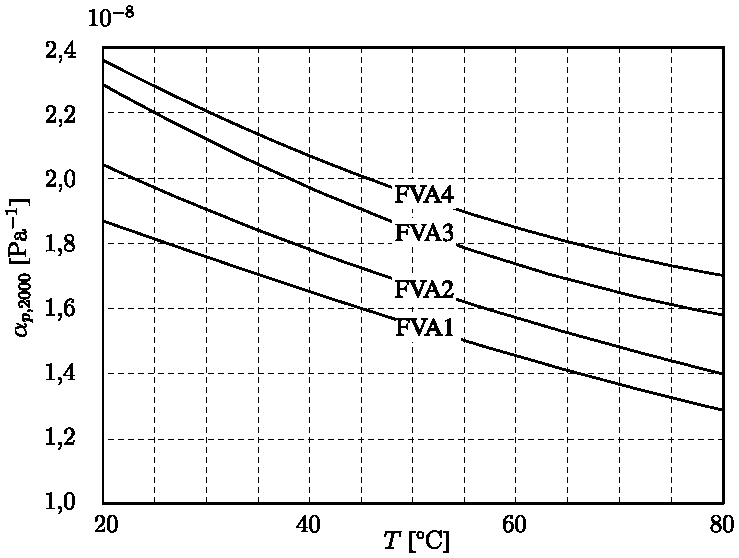
\includegraphics[]{./images/visko_druck_koeffizient.pdf}
    \caption{Verhalten des Druckkoeffizienten in Abhängigkeit von der Temperatur}
    \label{fig:druckkoeffizient_temperatur}
\end{figure}
\improvement[inline]{Figure quelle ???}
%

% ----------------------------------------
% Subsec: Dichte
% ----------------------------------------
\subsection*{Dichte}
\label{sub:dichte}

Für eine numerische Schmierfilmdickenmessung ist es notwendig zu wissen, wie die Dichte des Schmierstoffes unter verschiedenen Druck verhält.
Die Form des Schmierfilms kann nicht richtig berechnet werden, wenn diese Eigenschaft vernachlässigt wird.
Die Kompressibilität eines Schmierstoffes $C$ ist nach Chu und Cameron mit folgender Formel zu berechnen:
% ----------------------------------------
% Eq: Die Kompressibilität eines Schmierstoffes
% ----------------------------------------
\begin{equation}
    \label{eq:kompressibilitaet}
    C = \left( \frac{1}{\rho} \right) \frac{d\rho}{dp} = \left( \frac{1}{V} \right) \frac{dV}{dp}
\end{equation}
%
wobei V das Volumen und $dV$ die Änderung des Volumens ist.

Die Dichte der Mineralöle ist nach Hirano\cite{hirano} mit folgender Formel zu berechnen
% ----------------------------------------
% Eq: Dichte nach Hirano
% ----------------------------------------
\begin{equation}
    \label{eq:dichte_hirano}
    \rho = \rho_0 \left( 1 + \frac{0,6  p}{1 + 1,7  p} \right)
\end{equation}
%
wobei $p$ in $GPa$ und $\rho_0$ die Dichte beim normalen Luftdruck ($0,87~kg/m^3$ bei $20^\circ C$) ist.
% ----------------------------------------
% Fig: Druckkoeffizient der FVA-Referenzöle in Abhängigkeit von der Temperatur
% ----------------------------------------
\begin{figure}[htb]
    \centering
    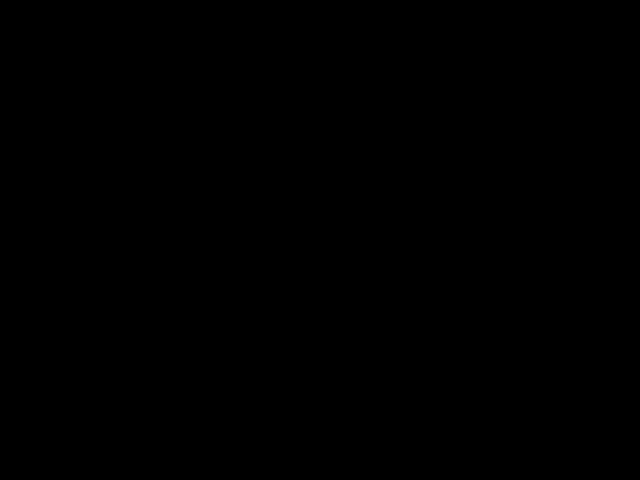
\includegraphics[width=5cm]{./images/blank_img.jpg}
    \caption{Variation der Dichte bei verschiedenen Drücke}
    \label{fig:variation_der_dichte_bei_verschiedenen_druecke}
\end{figure}

% ----------------------------------------
% Subsec: Brechungsindex
% ----------------------------------------
\subsection*{Brechungsindex}
\label{sub:brechungsindex}

Für die Messverfahren, die auf optischen Interferometrie basieren, braucht man die Abhängigkeit zwischen der Dichte und dem Brechungsindex des Schmierstoffes.
Nach Gohar wird das Verhältnis mit der Formel\ref{eq:dichte_brechnungsindex} beschrieben.
% ----------------------------------------
% Eq: Dichte und Brechungsindex
% ----------------------------------------
\begin{equation}
    \label{eq:dichte_brechnungsindex}
    c  p = \frac{n^2 - 1}{n^2 + 2}
\end{equation}
%
wobei $c$ ein Ölkonstante ist (zB: SAE30, $c = 0,33$).
Der Brechungsindex für meist Mineralöle bei normalen Luftdruck ist c.a 1,51.

% ----------------------------------------
% Subsec: Wärmeleitfähigkeit
% ----------------------------------------
\subsection*{Wärmeleitfähigkeit}
\label{waermeleitfaehigkeit}

Um die Temperaturerhöhung des Schmierstoffes unter Schubspannung zu schätzen, ist dessen Wärmeleitfähigkeit $k$ nötig.
Nach Cameron\cite{cameron} kann diese Größe beim normalen Luftdruck mit folgender Formel berechnet werden.
% ----------------------------------------
% Eq: Wärmeleitfähigkeit
% ----------------------------------------
\begin{equation}
    \label{eq:waermeleitfaehigkeit}
    k = \frac{0,1173 - 6,33 \times 10^{-5} \ T}{\rho_0}
\end{equation}
%
wobei $T$ die absolute Temperatur in $K$ und $\rho_0$ die Dichte in $kg/m^3$ ist.

% ----------------------------------------
% Subsec: Newtonsche Fluide
% ----------------------------------------
\subsection*{Newtonsche Fluide}
\label{sub:newtonsche_fluide}

Wenn die Viskosität eines Fluids von der Schubspannung unabhängig ist, wird das Fluid als newtonsches Fluid bezeichnet - Abbildung\ref{fig:newtonsche_fluide}.
Flüssigkeiten, deren Viskosität mit steigender Schubspannung zunimmt, nennt man dilatant.
Solches Verhalten ist geeignet für Suspensionen, nicht als Schmierstoff.
Strukturviskose Fluide sind die Umkehr der Dilatanz.
Strukturviskosität tritt bei synthetischen Fluiden auf.
Für die Bestimmung der Schmierfilmdicke werden alle Fluide in Rahmen dieser Arbeit als newtonsche Fluide angenommen.
% ----------------------------------------
% Fig: Newtonsche und nicht newtonsche Fluide
% ----------------------------------------
\begin{figure}[htb]
    \centering
    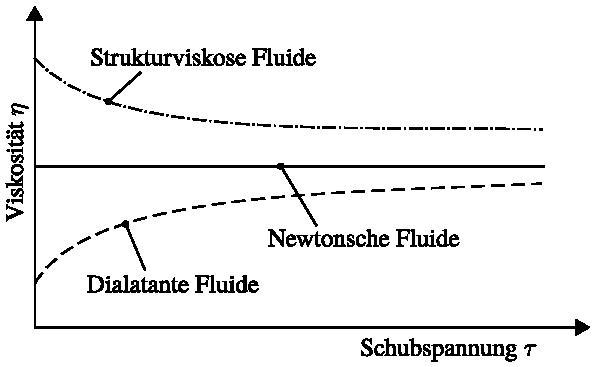
\includegraphics[]{./images/newtonsche_nichtnewtonsche_fluide.pdf}
    \caption{Newtonsche und die andere Fluide\cite{wisniewski}}
    \label{fig:newtonsche_fluide}
\end{figure}
%

% ----------------------------------------
% Sec: Reibung
% ----------------------------------------
\section{Reibung}
\label{sec:reibung}

% ----------------------------------------
% Subsec: Reibungsarten
% ----------------------------------------
\subsection{Reibungsarten}
\label{sub:reibungsarten}

Bewegungsreibung ist immer da, wo sich berührende Körper bzw. Stoffbereiche relativ zueinander bewegen.
Sie ist entgegen der Bewegungsrichtung gerichtet und wandelt die mechanische Energie in Wärme.
Man unterscheidet zwischen innerer und äußerer Reibung.
Äußere Reibung tritt auf, wo die Flächen der unterschiedlichen Körpern sich berühren.
Von innerer Reibung spricht man, wenn die sich berührenden Stoffbereiche einem Körper angehören, z.B im Schmierstoff.

Im Gegensatz zur Bewebungsreibung tritt die Haftreibung auf, wo es keine relative Bewegung zwischen Reibpartner gibt.
In diesem Fall ist angreifende Kraft nicht ausreichend, um die Körper in Bewegung zu bringen.

Reibung wird durch den Reibwert $\mu$ charakterisiert.
Er beschreibt das Verhältnis von Reibungskraft $F_R$ und der Normalkraft $F_N$
% ----------------------------------------
% Eq: Reibung
% ----------------------------------------
\begin{equation}
    \label{eq:reibung}
	\mu = \cfrac{F_R}{F_N}
\end{equation}
%

Die Bewegungsreibung kann man in drei Kategorien Gleitreibung, Rollreibung und Bohrreibung einteilen (Abbildung \ref{fig:arten_der_bewegungsreibung}).
In der Praxis treten meist Kombinationen dieser drei Reibungsarten auf.
Die wichtigste ist hier die sogenante Wälzreibung, eine Kombination aus Rollen und Gleiten.
% ----------------------------------------
% Fig: Arten der Bewegungsreibung
% ----------------------------------------
\begin{figure}[htb]
    \centering
    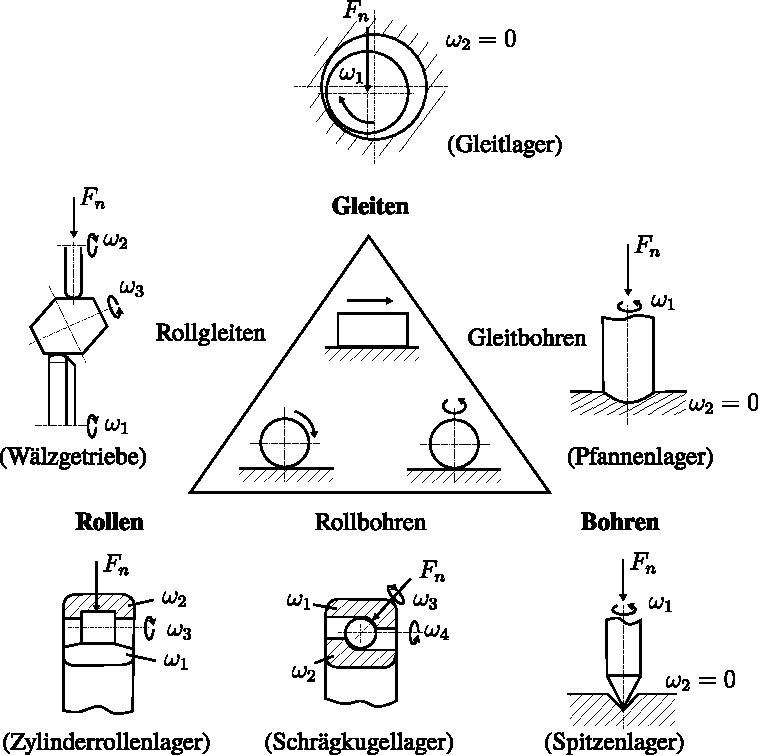
\includegraphics[]{./images/bewegungsarten.pdf}
    \caption{Arten der Bewegungsreibung \cite{steinhilper_2008}}
    \label{fig:arten_der_bewegungsreibung}
\end{figure}
%

% ----------------------------------------
% Subsec: Reibungszustände
% ----------------------------------------
\subsection{Reibungszustände}
\label{sub:reibungszustaende}

Die Reibungszustände werden durch den Kontaktzustand der beteiligten Reibpartner beschrieben.
Man spricht hier von Festkörper-, Grenz-, Misch-, Flüssigkeits- und Gasreibung.
Da die Gasreibung für diese Arbeit unrelevant ist, wird es kurz auf die einzelnen Reibungszustände außer Gasreibung eingegangen.

% ----------------------------------------
% Par: Festkörperreibung
% ----------------------------------------
\paragraph{Festkörperreibung}
\label{par:festkoerperreibung}
%
\begin{wrapfigure}{R}{0.25\textwidth}
    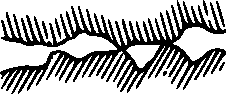
\includegraphics[trim={0 1cm 0 1cm}]{./images/festkoerperreibung.pdf}
\end{wrapfigure}

Von Festkörperreibung spricht man, wenn kein Schmierstoff sich im Reibkontakt befindet.
Dabei besteht die Gefahr bei hohen Flächenpressungen, dass die beiden Körper aneinander haften, verschleißen und es zum Fressen kommen kann.

% ----------------------------------------
% Par: Grenzreibung
% ----------------------------------------
\paragraph{Grenzreibung}
\label{par:grenzreibung}
%
\begin{wrapfigure}{R}{0.25\textwidth}
    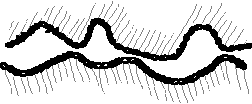
\includegraphics[trim={0 0.5cm 0 0.5cm}]{./images/grenzreibung.pdf}
\end{wrapfigure}

Grenzreibung ist von der Festkörperreibung schon sehr ähnlich.
Allerdings werden die Oberflächen der Reibpartner von einer Schicht getrennt und befinden sich nicht direkt in Berührung.
Diese Schicht kann zum Beispiel durch Oxidation, Adsorption oder chemische Reaktionen entstanden sein und vermindert die Reibung im Verleich zur Festkörperreibung schon eheblich.

% ----------------------------------------
% Par: Mischreibung
% ----------------------------------------
\paragraph{Mischreibung}
\label{par:mischreibung}
%
\begin{wrapfigure}{R}{0.25\textwidth}
    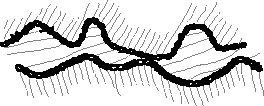
\includegraphics[trim={0 0.5cm 0 0.5cm}]{./images/mischreibung.pdf}
\end{wrapfigure}

Bei Mischreibung gibt es schon im Reibkontakt ein bisschen Schmierstoff und die Laufflächen werden zum Teil durch einen Schmierfilm getrennt.
Leider ist der nicht hoch genug, um ein vollständiges Trennen der beiden Körpern zu erreichen.
Es kommt immer noch die Berührung der Rauheitsspitzen der Laufflächen.
Die Reibung bei der Mischreibung ist deutlich geringer als die der Grenzreibung. Allerdings bleibt immer noch der Verschleiß im Reibkontakt.

% ----------------------------------------
% Par: Flüssigkeitsreibung
% ----------------------------------------
\paragraph{Flüssigkeitsreibung}
\label{par:fluessigkeitsreibung}
%
\begin{wrapfigure}{R}{0.25\textwidth}
    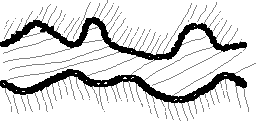
\includegraphics[trim={0 0.5cm 0 0.5cm}]{./images/fluessigkeitreibung.pdf}
\end{wrapfigure}

Bei Flüssigkeitsreibung handelt sich um eine vollständige Trennung der Laufflächen.
Selbst die Rauheitsspitzen berühren sich hierbei nicht mehr.
Die äußere Reibung ist weg, bleibt nur noch die innere Reibung, welche durch die Scherbeanspruchung des Schmierstoffs hervorgerufen wird.

Der Aufbau des Schmierfilms erfolgt hydrodynamisch, elastohydrodynamisch oder hydrostatisch.
Hydrostatisch aufgebaute Schmierfilme werden durch externe Aggregate wie zum Beispiel eine Pumpe aufgebaut.
Bei der hydrodynamischen Schmierung wird der Schmierfilm durch die Relativbewegung der Reibpartner aufgebaut.
Die hydrodynamische Schmierung tritt im Allgemein nur bei konformen Kontaktpaarungen.
Mit konformen Kontaktpaarungen spricht man von Kontaktkörpern, die sich auf eine Fläche berühren.
Eine Verformung der Oberflächen spielt hier keine wichtige Rolle, da die Pressungen aufgrund der großen Kontaktflächen vergleichsweise gering sind.
Im Gegenteil dazu ist bei der elastohydrodynamischen Schmierung die Flächenpressung ein entscheidender Faktor zum Aufbau einer tragenden Schicht.
Die Kontaktpaarungen bei dieser Schmierung sind im Allgemein kontraform.
Ihre Flächen berühren sich nur in einem Punkt oder einer Linie.
Dadurch treten deutlich höhere Flächenpressungen als bei konformen Kontakten, was zu einer lokalen Verformung der Oberflächen führt.
Durch dieses Phänomen und die Zunahme der Viskosität des Schmierstoffes unter hohem Druck wird der Schmierfilm im Kontaktbereich bei elastohydrodynamischen Schmierung aufgebaut.

% ----------------------------------------
% Par: Stribeck-Kurve
% ----------------------------------------
\subsection{Stribeck-Kurve}
\label{sub:stribeck-kurve}

Zur anschaulichen Darstellung der verschiedenen Reibungszustände wird häufig die Stribeck-Kurve gewählt.
In die Abbildung \ref{fig:stribeck-kurve} wird die Reibungszahl eines geschmierten Gleitlagers in Abhängigkeit von der Geschwindigkeit dargestellt.
% ----------------------------------------
% Fig: Stribeck-Kurve
% ----------------------------------------
\begin{figure}[htb]
    \centering
    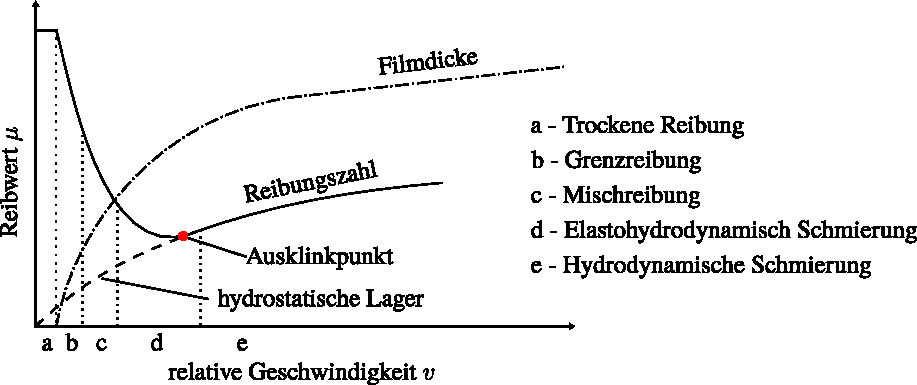
\includegraphics[]{./images/stribeckkurve.pdf}
    \caption{Stribeck-Kurve eines geschmierten Gleitlagers \cite{ikz_haustechnik}}
    \label{fig:stribeck-kurve}
\end{figure}
%

Im Stillstand tritt erst einmal reine Haftreibung auf.
Nach dem Anlauf des Lagers sinkt die Reibungszahl trotz des fehlenden Schmierstoffes im Reibkontakt und es kommt zur Grenzreibung.
Mit zunehmender Relativgeschwindigkeit zwischen Lagerbuchse und Welle wird der Schmierstoff in den Lagerspalt gefördert.
Jetzt nimmt die Reibung weiter ab und es kommt zur Mischreibung.
Bei weiter zunehmender Drehzahl sinkt die Reibungszahl ab bzw. steigt der Schmierfilm so weit an, bis es ab dem Ausklinkpunkt zur reinen Flüssigkeitsreibung kommt.
Nun schwimmt die Welle im Schmierstoff und berührt sich nicht mehr mit der Lagerbuchse.
Da die innere Reibung mit der steigenden Drehzahl zunimmt, liegt an der Stelle (Ausklinkpunkt) ein Minimum der Reibungszahl vor.

Für Gleitlager, deren Schmierfilm hydrostatisch durch eine Pumpe aufgebaut wird, gilt die Stribeck-Kurve nicht.
Da der Schmierfilm schon beim Stillstand voll ausgebildet ist, befinden sich solche Lager bei jeder Drehzahl im Bereich der Flüssigkeitsreibung.

% ----------------------------------------
% Sec: Betrachtung des EHD-Kontaktes
% ----------------------------------------
\section{Betrachtung des EHD-Kontaktes}
\label{sec:betrachtung_des_ehd_kontaktes}

Die Kontaktflächen von Maschinenelementen werden in zwei Grundformen eingeteilt.
Dies sind konforme (z.B. Gleitlager) und nichtkonforme Paarungen (z.B. Zahnrad, Reibrad, Nocken-Stößel).
Abbildung~\ref{fig:konforme_kontraforme_kontakte} zeigt die Beispiele konforme und nichtkonforme Kontakte.
% ----------------------------------------
% Fig: Nichtkonforme Paarungen
% ----------------------------------------
\begin{figure}[htb]
    \centering
    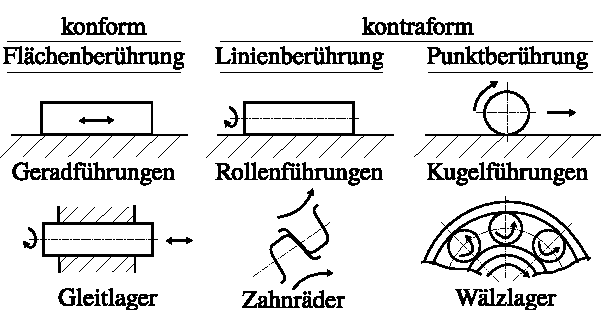
\includegraphics[]{./images/konforme_kontraforme_kontakte.pdf}
    \caption{Konforme und kontraforme Kontakte \cite{steinhilper_2008}}
    \label{fig:konforme_kontraforme_kontakte}
\end{figure}
%
Gegenteil zu den konformen Kontakten, wo die Pressungen in der Größenordnung von $10 MPa$ auftreten, können in zwischen den Laufflächen nichtkonformer Kontakt die Druckspannungen 0,5 GPa und höher betragen.
Durch die enorme, konzentrierte Belastung werden die Flächen an dem Kontaktpunkt elastisch verformt und vergrößert.
Im Folgenden soll der Wälzkontakt nach Wisniewski\cite{wisniewski} näher betrachtet werden.

\subsection{Kontakt von beliebig gekrümmten Elementen}
\label{sub:kontakt_von_beliebig_gekruemmten_elementen}

Bei der Betrachtung des konzentrischen Kontaktes werden alle Oberflächen als ideal glatt angenommen und durch deren minimalen und maximalen Krümmungen wird die Geometrie des Grundkörpers bzw. des Gegenkörpers beschrieben.
Beim konvexen Körper (Index 1) sind die Krümmungsradien ($r_{11}, r_{12}$) positiv und beim konkaven Körper (Index 2) sind die Radien ($r_{21}, r_{22}$) negativ.
Zwischen den beiden Ebenen, die $r_{11}$ und $r_{21}$ erhalten, bildet sich der Winkel $\varphi$.
In Abbildung~\ref{fig:kontaktgeometrie_nichtkonforme_kontakte} wird die generelle Kontaktgeometrie bei nicht konformen Festkörpern dargestellt.
% ----------------------------------------
% Fig: Wälzkontakt nach Wisniewski
% ----------------------------------------
\begin{figure}[htb]
    \centering
    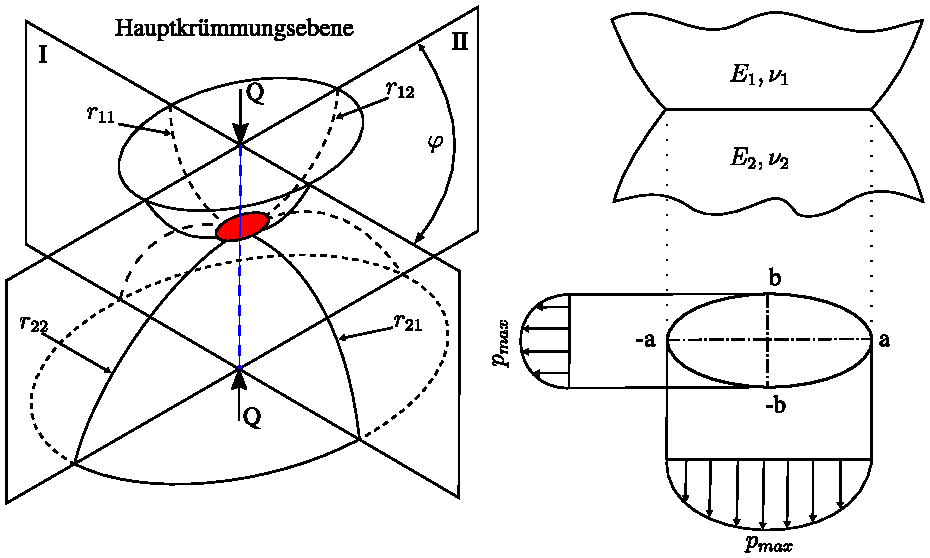
\includegraphics[width=0.8\textwidth]{./images/Hertzsche_Pressung.pdf}
    \caption{Kontaktgeometrie bei nicht konformer Paarungen\cite{psm}}
    \label{fig:kontaktgeometrie_nichtkonforme_kontakte}
\end{figure}
%
Im Kontaktpunkt bildet sich die Kontaktflächen eine Ellipse mit den Halbachsen $a$ und $b$.
Zu $a$ und $b$ zu bestimmen, braucht man das reduzierte Elastizitätsmodul $E$, die Belastung $P$ und der Krümmungsradius $R$.
% ----------------------------------------
% Eq: Laengen der Halbachsen der Kontaktellipse
% ----------------------------------------
\begin{align}
    a = \beta_a  \sqrt[3]{\frac{3  P  R}{E}} \label{eq:laenge_a} \\
    b = \beta_b  \sqrt[3]{\frac{3  P  R}{E}} \label{eq:laenge_b}
\end{align}
%
Der reduzierte Elastizitätsmodul $E$ beschreibt die elastische Eigenschaften der beiden Elemente und wird definiert als
% ----------------------------------------
% Eq: Der reduzierte Elastizitätsmodul E
% ----------------------------------------
\begin{equation}
    \label{eq:reduzierter_elastizitaetsmodul}
    \frac{1}{E} = \frac{1}{2}  \left( \frac{1 - \nu_1^2}{E_1} + \frac{1 - \nu_2^2}{E_2} \right)
\end{equation}
%
wobei $\nu_x$ die Querkontraktionszahl der Kontaktkörper und $E_x$ der Elastizitätsmodul der Kontaktkörper ist.
Die Druckverteilung $p$ hat eine Form eines Halbellipsoids und wird so definiert
% ----------------------------------------
% Eq: Druckverteilung p
% ----------------------------------------
\begin{equation}
    \label{eq:druckverteilung}
    p = p_0  \sqrt{1 - \left( \frac{x}{b} \right)^2 - \left( \frac{y}{a} \right)^2}
\end{equation}
%
wobei $x, y$ die Koordinaten in der Ebene und die maximale Pressung $p_0$ ein Produkt der Belastung $P$ und der Länge von Halbachsen $a, b$ sind.
% ----------------------------------------
% Eq: Maximale Pressung p0
% ----------------------------------------
\begin{equation}
    \label{eq:maximale_pressung}
    p_0 = \frac{3  P}{2  \pi  a  b}
\end{equation}
%
Der reziproke Krümmungsradius $R$ wird mit der Summe aller vier Hauptkrümmungen $r_x$ bestimmt
% ----------------------------------------
% Eq: Krümmungsradius R
% ----------------------------------------
\begin{equation}
    \label{eq:kruemmungsradius}
    \frac{1}{R} = \frac{1}{r_{11}} + \frac{1}{r_{12}} + \frac{1}{r_{21}} + \frac{1}{r_{22}}
\end{equation}
%
Die Koeffizienten $\beta_a$ und $\beta_b$ zur Bestimmung der Berührungsfläche in einem konformen Kontakt kann über den Parameter $\cos{\psi}$ aus dem Diagram~\ref{fig:beta_a_und_beta_b_als_funktion_der_cos_psi} abgelesen werden.
% ----------------------------------------
% Fig: beta_a und beta_b als Funktion des cos_psi
% ----------------------------------------
\begin{figure}[htb]
    \centering
    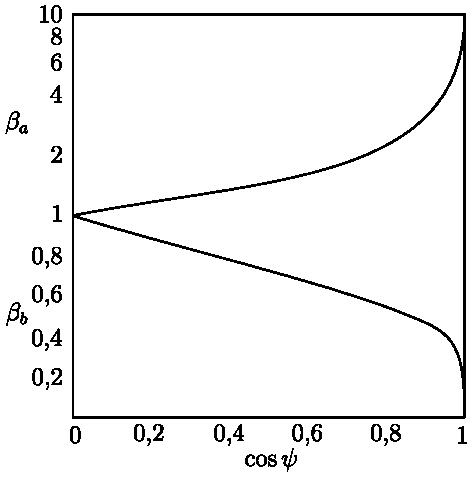
\includegraphics[]{./images/beta_cos_psi_diagram.pdf}
    \caption{$\beta_a$ und $\beta_b$ als Funktion von $\cos{\psi}$\cite{wisniewski}}
    \label{fig:beta_a_und_beta_b_als_funktion_der_cos_psi}
\end{figure}
%

Der Parameter $\cos{\psi}$ kann mit folgender Formel\ref{eq:cos_psi} berechnet werden
% ----------------------------------------
% Eq: cos psi
% ----------------------------------------
\begin{equation}
    \label{eq:cos_psi}
    \cos{\psi} = R  \sqrt{\left( \frac{1}{r_{11}} - \frac{1}{r_{12}} \right)^2 
                                + \left( \frac{1}{r_{21}} - \frac{1}{r_{22}} \right)^2 
                                + 2  \cos{2 \varphi} 
                                 \left( \frac{1}{r_{11}} - \frac{1}{r_{12}}  \right)^2 
                                 \left( \frac{1}{r_{21}} - \frac{1}{r_{22}} \right)^2}
\end{equation}
%

Für ein Kugel-Scheibe-Modell gilt
%
\begin{align*}
    r_{11} &= r_{12} = r_{Kugel} \\
    r_{21} &= r_{22} = r_{Scheibe} = \infty
\end{align*}
%

% ----------------------------------------
% Sec: Schmierung nach Hamrock und Dowson
% ----------------------------------------
\section{Schmierfilmdicke nach Hamrock und Dowson}
\label{sec:schmierfilmdicke_nach_hamrock_und_dowson}

Die Berechnung der Schmierfilmhöhe bei EHD-Schmierung wurde von vielen Autoren behandelt und ihre Ergebnisse wurden von Dowson und Higginson mit numerischer Unterstützung bestätigt.
Nach Dowson und Higginson kann die Schmierfilmdicke durch vier dimensionslose Größe ermittelt werden.
% ----------------------------------------
% Eq: Allgemein Schmierfilmdicke
% ----------------------------------------
\begin{equation}
    \label{eq:allgemein_schmierfilmdicke}
    H = k G^{\alpha} U^{\beta} W^{\gamma}
\end{equation}
%
wobei

% ----------------------------------------
% List: Parameter zur Berechnung der Schmierfilmdicke
% ----------------------------------------
\begin{tabular}{lll}
    Schmierfilmparameter & $H_{min} = \cfrac{h_{min}}{R} ;\quad H_0 = \cfrac{h_0}{R}$ & (c.a $10^{-6} \rightarrow 10^{-2}$) \\
    Werkstoffparameter & $G = \alpha_p E$ & (c.a $2000 \rightarrow 6000$) \\
    Geschwindigkeitsparameter & $U = \cfrac{\eta_0 u}{E R}$ & (c.a $10^{-13} \rightarrow 10 ^{-8}$) \\
    Belastungsparameter & $W = \cfrac{P}{E R}$ & (c.a $10^{-5} \rightarrow 10^{-3}$)
\end{tabular}
%

In einer Reihe von Veröffentlichungen in \cite{hamrock_dowson_1976_a}\cite{hamrock_dowson_1976_b}\cite{hamrock_dowson_1977_a}\cite{hamrock_dowson_1977_b} wurde von Dowson und Hamrock die Formel zur Berechnung der minimalen und zentralen Schmierfilmdicke in elliptischen Punktkontakten angeführt.
% ----------------------------------------
% Eq: Schmierfilmdicke von Dowson und Hamrock
% ----------------------------------------
\begin{align}
    \label{eq:mininmale_schmierfilmdicke_downson_hamrock}
    H_{min} &= \cfrac{3,63 G^{0,49} U_0^{0,68}}{W_0^{0,073}} (1 - e^{-0,68 \chi}) \\
    \label{eq:zentrale_schmierfilmdicke_downson_hamrock}
    H_0 &= \cfrac{2,69 G^{0,53} U_0^{0,67}}{W_0^{0,067}} (1 - 0,61 e^{-0,73 \chi}) \\
    \text{mit} \quad
    U_0 &= \cfrac{\eta_0 u}{E R_x};\ 
    W_0 = \cfrac{P}{E R_x^2};\
    \chi = \frac{a}{b};\
    \frac{1}{R_x} = \frac{1}{R_{1x}} + \frac{1}{R_{2x}} \nonumber 
\end{align}
%
wobei $\chi$ das Verhältnis der Halbachsen der Kontaktellipse ist und $R_x$ bedeutet der Krümmungsradius in der Bewegungsebene.
Der Geschwindigkeits-, und Belastungsparameter weichen hier von den verallgemeinerten ab.

Man kann hier erkennen, dass der Geschwindigkeitsparameter $U_0$ mit einem Exponenten von $0,67$ den höchsten Einfluss auf die Schmierfilmdicke hat.
Erstaunlicherweise hat die Belastung kaum den Einfluss.
